\documentclass[border=6pt]{standalone}
\usepackage[T1]{fontenc}
\usepackage[utf8]{inputenc}
\usepackage[scaled=0.98]{helvet}
\renewcommand{\familydefault}{\sfdefault}
\usepackage{amsmath}
\usepackage{graphicx}
\graphicspath{{../../../../../../exercises_lecturenotes/lecture_notes/kurs100_lektionsnoter/}}
\usepackage{tikz}
\usepackage{pgfplots}
\pgfplotsset{compat=1.18}
\usetikzlibrary{arrows.meta, decorations.pathreplacing, calc, positioning, fit, backgrounds, shapes.geometric}
\usepgfplotslibrary{groupplots,fillbetween}
\definecolor{scanpink}{HTML}{E5006D}
\definecolor{scanteal}{HTML}{00A6A6}
\definecolor{scannavy}{HTML}{243746}
\definecolor{scanlightgray}{HTML}{F1F2F3}
\definecolor{ScanBlue}{RGB}{24,73,169}
\definecolor{ScanGreen}{RGB}{55,140,75}
\definecolor{ScanOrange}{RGB}{235,120,40}
\definecolor{ScanDark}{RGB}{45,45,45}
\definecolor{ScanGray}{RGB}{130,130,130}
\begin{document}
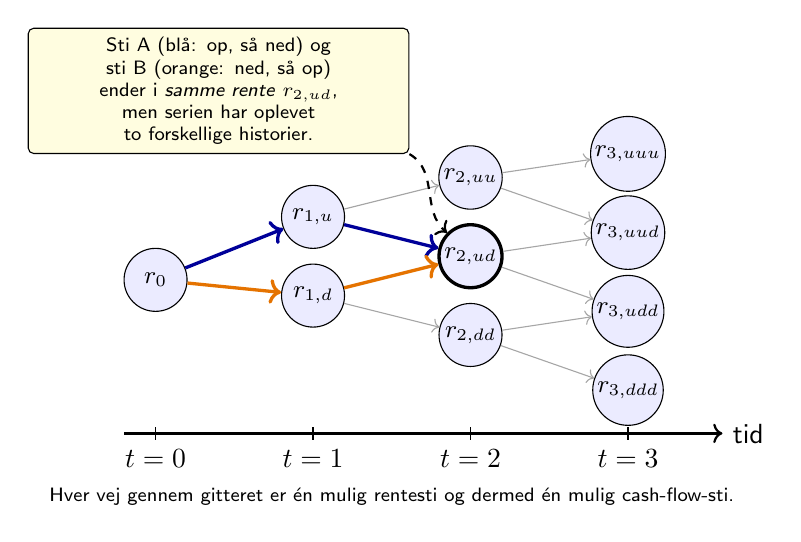
\begin{tikzpicture}[
    rate/.style={circle, draw, fill=blue!8, minimum size=8mm, inner sep=1pt, font=\small},
    note/.style={draw, rounded corners=2pt, fill=yellow!12, align=center, text width=46mm, font=\scriptsize},
    arr/.style={->, thin, gray!70},
    stiA/.style={->, very thick, blue!60!black},
    stiB/.style={->, very thick, orange!90!black}
]

% placering af tidsakse
\def\axisy{-1.95}

% tidsakse
\draw[->, thick] (-0.4,\axisy) -- (7.2,\axisy) node[right] {tid};
\foreach \x/\lab in {0/{\(t=0\)},2/{\(t=1\)},4/{\(t=2\)},6/{\(t=3\)}} {
    \draw (\x,\axisy-0.08) -- (\x,\axisy+0.08);
    \node[below] at (\x,\axisy-0.08) {\lab};
}

% knuder
\node[rate] (n00) at (0,0) {\(r_0\)};
\node[rate] (n11) at (2,0.8) {\(r_{1,u}\)};
\node[rate] (n10) at (2,-0.2) {\(r_{1,d}\)};
\node[rate] (n22) at (4,1.3) {\(r_{2,uu}\)};
\node[rate, very thick] (n21) at (4,0.3) {\(r_{2,ud}\)};
\node[rate] (n20) at (4,-0.7) {\(r_{2,dd}\)};
\node[rate] (n33) at (6,1.6) {\(r_{3,uuu}\)};
\node[rate] (n32) at (6,0.6) {\(r_{3,uud}\)};
\node[rate] (n31) at (6,-0.4) {\(r_{3,udd}\)};
\node[rate] (n30) at (6,-1.4) {\(r_{3,ddd}\)};

% almindelige grene
\draw[arr] (n11) -- (n22);
\draw[arr] (n10) -- (n20);
\draw[arr] (n22) -- (n33);
\draw[arr] (n22) -- (n32);
\draw[arr] (n21) -- (n32);
\draw[arr] (n21) -- (n31);
\draw[arr] (n20) -- (n31);
\draw[arr] (n20) -- (n30);

% de to fremhævede stier
\draw[stiA] (n00) -- (n11);
\draw[stiA] (n11) -- (n21);
\draw[stiB] (n00) -- (n10);
\draw[stiB] (n10) -- (n21);

% forklaring
\node[note] (annotation) at (0.8,2.4)
{Sti A (blå: op, så ned) og sti B (orange: ned, så op)\\
ender i \emph{samme rente} \(r_{2,ud}\),\\
men serien har oplevet to forskellige historier.};
\draw[->, thick, dashed] (annotation.south east) to[out=-30,in=140] (n21.north west);

\node[align=center, font=\scriptsize] at (3,-2.75)
{Hver vej gennem gitteret er én mulig rentesti og dermed én mulig cash-flow-sti.};

\end{tikzpicture}
\end{document}
